\documentclass[manuscript]{acmart}

\usepackage{amsmath}
\usepackage{booktabs}
\usepackage{tabularx}
\usepackage{multirow}
\usepackage{tikz}
\usetikzlibrary{arrows.meta,positioning,fit,matrix}
\usepackage{pgfplots}
\usepgfplotslibrary{groupplots}
\pgfplotsset{compat=1.18}

\acmJournal{TOMM}
\title{NARCIS: Authenticated Neural Coverless Image Signaling with Attack-Qualified Codebooks and Error Correction}

\author{Arthur Ulrich Ewane}
\orcid{0009-0001-6722-2842}
\affiliation{\institution{Department of Computer Science, University of Yaound\'e I, LIRIMA, TEAM GRIMCAPE}\city{Yaound\'e}\country{Cameroon}}
\email{ulrich.ewane@facsciences-uy1.cm}

\author{Juvet Karnel Sadi\'e}
\affiliation{\institution{Department of Computer Science, University of Yaound\'e I, LIRIMA, TEAM GRIMCAPE}\city{Yaound\'e}\country{Cameroon}}
\affiliation{\institution{UMMISCO, IRD France Nord}\city{Bondy}\country{France}}
\affiliation{\institution{Sorbonne Universit\'e, UMI 209 UMMISCO}\city{Paris}\country{France}}
\email{sadie.juvet@gmail.com}

\author{St\'ephane Ga\"el R. Ekodeck}
\orcid{0000-0002-8094-8832}
\affiliation{\institution{Department of Computer Science, University of Yaound\'e I, LIRIMA, TEAM GRIMCAPE}\city{Yaound\'e}\country{Cameroon}}
\affiliation{\institution{UMMISCO, IRD France Nord}\city{Bondy}\country{France}}
\affiliation{\institution{Sorbonne Universit\'e, UMI 209 UMMISCO}\city{Paris}\country{France}}
\email{stephane-gael.ekodeck@facsciences-uy1.cm}

\author{Serge Alain Eb\'el\'e}
\orcid{0000-0001-7036-7068}
\affiliation{\institution{Department of Computer Science, University of Yaound\'e I, LIRIMA, TEAM GRIMCAPE}\city{Yaound\'e}\country{Cameroon}}
\affiliation{\institution{UMMISCO, IRD France Nord}\city{Bondy}\country{France}}
\affiliation{\institution{Sorbonne Universit\'e, UMI 209 UMMISCO}\city{Paris}\country{France}}
\email{serge-alain.ebele@facsciences-uy1.cm}

\author{Vivien Lo\"ick Beyala Kamgang}
\orcid{0000-0002-3644-1866}
\affiliation{\institution{RTU Mathematics and Computer Science, The University of Bertoua}\city{Bertoua}\country{Cameroon}}
\affiliation{\institution{RUFCEA (UR-IFIA), University of Dschang}\city{Dschang}\country{Cameroon}}
\email{vivsxx@univ-bertoua.cm}

\author{Damaris Belle M. Fotso}
\orcid{0009-0001-8736-0644}
\affiliation{\institution{Department of Computer Science, University of Yaound\'e I, LIRIMA}\city{Yaound\'e}\country{Cameroon}}
\email{makwate.fotso@facsciences-uy1.cm}

\author{Chantal Marguerite Mveh-Abia}
\orcid{0009-0005-9398-1067}
\authornote{Corresponding author.}
\affiliation{\institution{Department of Computer Science, University of Yaound\'e I, LIRIMA, TEAM GRIMCAPE}\city{Yaound\'e}\country{Cameroon}}
\affiliation{\institution{Department of Computer Engineering, National Advanced School of Engineering, University of Yaound\'e I}\city{Yaound\'e}\country{Cameroon}}
\email{cmmveh@yahoo.fr}

\renewcommand{\shortauthors}{Ewane et al.}

\begin{abstract}
Selection-based coverless communication preserves carrier pixels while reliability and statistical inconspicuousness depend on the selected-index distribution and the image channel. We present NARCIS, an authenticated neural coverless image-signaling protocol that treats finite-index feasibility, channel robustness, session balancing, and selection detectability as joint protocol constraints. NARCIS combines a learned normalized image descriptor, calibration-locked quantile codebooks, complementary five-cover group banks, exact session-balanced keyed Gray mapping, AES-GCM authenticated framing, replay control, and Reed--Solomon correction. The final operating point ($K=8$, group size 5, 128 Reed--Solomon parity bytes) was fixed on BOSSBase development evidence before external evaluation on five Caltech-101 partitions. The development lineage achieved 1,800/1,800 calibration recoveries across five seeds while exercising essentially the full index. External Caltech calibration recovered 1,800/1,800 authenticated messages. Eight unseen holdout transformations yielded 1,163/1,200 recoveries (96.92\%); the 37 failures were concentrated in the 12\% central-crop condition, while each of the other seven holdouts achieved 150/150. A repeated image-disjoint detector audit yielded mean macro-AUC 0.504 for SRM-lite/ExtraTrees, 0.513 for GLCM/logistic regression, and 0.527 for a 30-head CNN, supporting a low but measurable selection-leakage characterization. A frozen execution of the official DiffStega benchmark completed all 100 UniStega cases; independently reproduced correct-recovery PSNR reached 23.274 dB versus 23.290 dB in the original paper. Family-specific metrics preserve the distinct semantics of generated-image reconstruction and authenticated finite-index byte signaling.
\end{abstract}

\ccsdesc[500]{Security and privacy~Cryptography}
\ccsdesc[500]{Information systems~Multimedia information systems}
\ccsdesc[300]{Computing methodologies~Neural networks}
\keywords{coverless image steganography, cover selection, covert communication, multimedia security, authenticated encryption, error correction, steganalysis}

\begin{document}
\maketitle

\section{Introduction}
\label{sec:intro}

Image steganography traditionally hides information by modifying a carrier, whereas coverless approaches communicate through selection, indexing, semantic mapping, or generation. Selection preserves the original pixels, shifting the principal security question toward the distribution of transmitted images and the reliability of their labels after channel perturbations. Recent surveys accordingly separate cover-selection design from detectability and emphasize evaluation criteria that reflect the selected-carrier distribution \cite{azam2025coversurvey,kombrink2025survey}.

A finite shared index adds a second protocol constraint. Every protected message induces a concrete multiplicity demand over codebook symbols. Robust communication therefore requires enough qualified carrier groups for every requested symbol across the complete protected envelope. Stability-aware quantization and representative selection improve robust cover choice \cite{guo2026capacity}, while restoration and deep-hashing methods strengthen geometric robustness \cite{meng2025restoration,tan2026hashing}. NARCIS complements these directions by placing finite-index feasibility, authenticated message recovery, and selection detectability inside one end-to-end evaluation unit.

NARCIS couples a channel-aware quantile codebook with complementary five-cover groups whose majority-failure signatures are characterized on calibration transformations. A proportional-deficit scheduler preserves the natural signature mixture of each label bank, while an exact cyclic keyed Gray mapping balances coded symbols across visual clusters over every full $K$-session cycle. AES-GCM binds payload and session state, Reed--Solomon coding absorbs residual byte errors, and authenticated plaintext recovery becomes the final success criterion. The scientific contribution is this integrated finite-index construction and its externally frozen evaluation rather than any individual standard primitive.

The validation separates development evidence from external evidence. BOSSBase 1.01 \cite{bas2011boss} supports design and operating-point selection. The final protocol then evaluates Caltech-101 \cite{feifei2004caltech101,caltech101data} with $K=8$, five covers per coded symbol, 128 Reed--Solomon parity bytes, and 30 authenticated sessions per partition. The external campaign combines twelve calibration transformations, eight unseen holdout transformations, complete-index usage measurements, and repeated selection-steganalysis with SRM-lite, GLCM, and CNN detectors. A frozen execution of DiffStega \cite{yang2024diffstega} supplies an executable recent reference under its native reconstruction metrics.

The resulting evidence is broad across robustness, usage, and detectability. The BOSSBase development lineage achieves 1,800/1,800 calibration recoveries over five seeds, with 7,995--8,000 unique covers exercised per seed and mean repeated-session detector AUCs close to chance. On the external Caltech partitions, calibration reaches 1,800/1,800 authenticated recoveries and exercises all 7,000 covers in every partition. Unseen holdouts reach 1,163/1,200 authenticated recoveries (96.92\%), with the strongest 12\% crop defining the observed channel boundary. Final mean macro-AUCs are 0.504 for SRM-lite, 0.513 for GLCM, and 0.527 for the CNN. DiffStega completes all 100 official UniStega cases, with independently reproduced correct-recovery PSNR of 23.274 dB compared with 23.290 dB in the reference paper. Together, these results support strong bounded channel robustness and low measurable selection leakage under the evaluated threat model.

\section{Related Work and Positioning}
\label{sec:related}

\subsection{Selection, retrieval, and robust coverless communication}

Natural-image coverless schemes use block statistics, retrieval descriptors, object semantics, hashing, and learned features to map messages to carriers. Multi-object recognition \cite{luo2021multiobject} and joint selection/generation designs such as JoCS \cite{ren2024robust} illustrate the diversity of communication objects and mapping rules. Guo and Ping \cite{guo2026capacity} are especially close in spirit: their stability-aware pseudo-Zernike quantization and representative selection explicitly balance robustness and nominal capacity. NARCIS focuses on the complementary finite-index question: whether the complete authenticated coded demand can be realized by a fixed shared index and recovered at the plaintext level.

Geometric perturbations remain a central robustness challenge. Meng et al. \cite{meng2025restoration} restore attacked images before the underlying coverless decoder, while Tan et al. \cite{tan2026hashing} use deep unsupervised hashing to improve resistance to geometric attacks. NARCIS incorporates calibration transformations directly into codebook and group-bank construction, while eight stronger/intermediate values remain holdouts. The observed 12\% crop boundary therefore becomes an explicit external-validity result.

\subsection{Generative steganography and multimedia security}

Generative approaches communicate through synthesized content. DiffStega reconstructs a secret image through prompt- and password-conditioned diffusion \cite{yang2024diffstega}. Guidance-feature-distribution steganography embeds information in a generative feature distribution \cite{sun2024guidance}, and progressive generative steganography in TOMM jointly studies capacity, extraction, and detectability during high-resolution generation \cite{zhou2025pgs}. NARCIS operates on an indexed natural-image carrier set and measures exact authenticated byte recovery. The article therefore reports each family with its native information object and metrics.

Authentication also has several multimedia meanings. FaceSigns \cite{neekhara2024facesigns} embeds semi-fragile authentication information into media. NARCIS keeps indexed covers unchanged and authenticates the protected payload and session state, providing a complementary carrier-preserving authentication model.

\subsection{Steganalysis of selection policies}

Selection steganalysis tests whether the emitted subset differs statistically from the available carrier population. CNN-based image steganalysis can exploit subtle distributional differences \cite{li2023siairnet}; adversarial embedding work likewise shows that the evaluated steganalyst materially shapes the security conclusion \cite{wang2024adversarial}. Cao, Wang, and Zhang analyze cover-selection steganography directly and show that texture statistics can expose selection bias \cite{cao2025glcm}. NARCIS therefore evaluates the selected-vs.-remainder distinction with residual, texture, and learned detectors under image-disjoint train/test splits.

\begin{table}[t]
\caption{Positioning of representative recent approaches. Each row retains the semantics of its native communication object and evaluation protocol.}
\label{tab:positioning}
\small
\begin{tabularx}{\textwidth}{@{}lXXX@{}}
\toprule
Approach & Carrier / information object & Robustness mechanism & Security/evaluation emphasis \\
\midrule
Guo--Ping \cite{guo2026capacity} & Selected natural images / symbols & Stable PZM quantization and representative selection & Robustness and nominal capacity \\
Meng et al. \cite{meng2025restoration} & Existing coverless schemes & Attack classification and image restoration & Geometric robustness \\
DiffStega \cite{yang2024diffstega} & Generated images / secret image & Diffusion inversion/reconstruction & Perceptual recovery, password sensitivity, steganalysis \\
NARCIS & Unchanged indexed natural images / authenticated byte string & Calibration-locked codebook, complementary group bank, RS128 & Finite-index feasibility, exact authenticated recovery, selection detectability \\
\bottomrule
\end{tabularx}
\end{table}

\section{System and Threat Model}
\label{sec:threat}

\subsection{Parties and shared state}

Sender and receiver share an indexed image corpus $\mathcal{I}=\{x_i\}_{i=1}^{N}$, the trained descriptor and frozen codebook, and independent cryptographic subkeys for payload encryption, cluster mapping, and cover selection. The sender transmits existing indexed images unchanged. Session metadata records the authenticated sequence number, codebook size, padding information, and cover count. The implementation seals metadata with AES-GCM and binds it to sender/receiver identities.

The benchmark uses deterministic public key/nonce derivation to make every run reproducible. A production deployment can replace this benchmark root with an operational key-management service while preserving the protocol interfaces. For a partition key $K_{\mathrm{master}}$, HMAC-SHA256 derives subkeys for encryption, mapping, and selection. The benchmark nonce combines a four-byte HMAC-derived prefix with the unique 64-bit session sequence, giving explicit nonce uniqueness for sequences $0,\ldots,29$ under a fixed benchmark key.

\subsection{Channel and warden}

The image channel applies lossy compression, additive Gaussian noise, blur, resizing, central cropping, and small rotations. Calibration and holdout transformation values are disjoint. The receiver decodes directly from the received image stream under the declared channel family.

For detectability, we use a strong matched-index warden: for each authenticated session, images selected by that session form the positive class and the remaining images in the same frozen index form the negative class. Training and test image identities are disjoint. This measures selection leakage relative to the shared index distribution. The present scope focuses on image-content discrimination; sequence-level traffic features, temporal metadata, semantic profiling, and cross-platform behavioral traces define complementary future threat models.

\subsection{Security goals and claim boundary}

NARCIS separates cryptographic protection from empirical carrier-selection security. AES-GCM provides payload confidentiality/integrity and metadata authentication under its standard AEAD assumptions and nonce discipline \cite{nistgcm}; the replay guard rejects sequence numbers at or below the highest accepted value for a sender. Reed--Solomon coding \cite{reed1960polynomial} corrects residual byte errors within its decoding budget. Selection leakage is measured independently through the detector battery, while traffic-analysis resistance and broader steganographic secrecy belong to a larger deployment threat model.

\section{NARCIS Protocol}
\label{sec:method}

\begin{figure}[t]
\centering
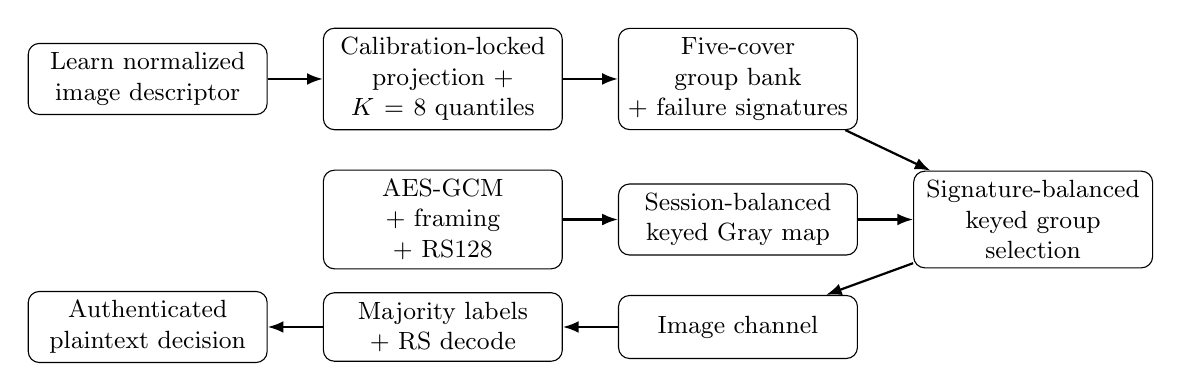
\begin{tikzpicture}[
  node distance=5mm and 7mm,
  box/.style={draw,rounded corners,align=center,minimum height=8mm,text width=28mm,font=\small},
  arrow/.style={-{Latex[length=2mm]},thick}
]
\node[box] (train) {Learn normalized\\image descriptor};
\node[box,right=of train] (project) {Calibration-locked\\projection + $K=8$ quantiles};
\node[box,right=of project] (bank) {Five-cover group bank\\+ failure signatures};
\node[box,below=of project] (crypto) {AES-GCM + framing\\+ RS128};
\node[box,right=of crypto] (map) {Session-balanced\\keyed Gray map};
\node[box,right=of map] (select) {Signature-balanced\\keyed group selection};
\node[box,below=of map] (channel) {Image channel};
\node[box,left=of channel] (decode) {Majority labels\\+ RS decode};
\node[box,left=of decode] (auth) {Authenticated\\plaintext decision};
\draw[arrow] (train)--(project);
\draw[arrow] (project)--(bank);
\draw[arrow] (crypto)--(map);
\draw[arrow] (map)--(select);
\draw[arrow] (bank)--(select);
\draw[arrow] (select)--(channel);
\draw[arrow] (channel)--(decode);
\draw[arrow] (decode)--(auth);
\end{tikzpicture}
\caption{NARCIS separates offline channel-aware index construction (top) from online protected transmission and recovery (bottom). The external-validation operating point is frozen before Caltech-101 outcomes are inspected.}
\Description{A block diagram showing descriptor learning, projection and quantile codebook construction, five-cover group banks, AES-GCM and Reed-Solomon framing, keyed Gray mapping, keyed group selection, the image channel, majority decoding, and final authentication.}
\label{fig:pipeline}
\end{figure}

\subsection{Invariant descriptor}

A convolutional encoder $f_\theta$ maps an image to an $L_2$-normalized descriptor $z=f_\theta(x)\in\mathbb{R}^{64}$. The frozen encoder contains four convolutional blocks with batch normalization and SiLU activations, adaptive average pooling, and a two-layer projector. Training uses paired channel augmentations and variance--invariance--covariance regularization in the spirit of VICReg \cite{bardes2022vicreg}. In the external campaign, images are fit to 256$\times$256 RGB at the channel boundary and 128$\times$128 at the encoder boundary; base width is 16, batch size 16, and training lasts five epochs with AdamW ($10^{-3}$ learning rate, $10^{-5}$ weight decay).

\subsection{Calibration-locked codebook and qualification}

For a candidate unit direction $u$, each indexed image receives scalar score
\begin{equation}
  s_i = u^\top f_\theta(x_i).
\end{equation}
A balanced one-dimensional quantile codebook partitions the clean scores into $K=8$ labels. Candidate projections comprise the first 16 clean-descriptor principal directions and 32 deterministic random directions. Projection selection uses the twelve calibration transformations: JPEG qualities 80 and 50; Gaussian noise standard deviations 5 and 12; Gaussian blur radii 0.8 and 1.5; resize scales 0.75 and 0.50; central crops 5\% and 10\%; and rotations 3 and 7 degrees.

Let $y_i$ be the clean label and $y_{i,a}$ the label under calibration attack $a$. Define correctness
\begin{equation}
 c_{i,a}=\mathbb{1}[y_{i,a}=y_i].
\end{equation}
The final protocol exploits complementary error patterns across covers. Projection candidates are ranked by analytical lower bounds on unavoidable majority-failing groups, followed by stable-cover and distribution-balance diagnostics. Holdout transformations, semantic category labels, detector outcomes, and final plaintext-recovery outcomes remain reserved for later validation stages.

\subsection{Complementary group bank}

Within each codebook label, all covers of the 7,000-image index carrying that label are partitioned into disjoint groups of five. A group $G$ fails calibration attack $a$ when fewer than three members retain their clean label:
\begin{equation}
 F_a(G)=\mathbb{1}\!\left[\sum_{i\in G} c_{i,a}<3\right].
\end{equation}
The vector $(F_a(G))_a$ is stored as a calibration majority-failure signature. Group-bank construction minimizes majority-failing group/attack cells using deterministic restarts and swap proposals, and compares the achieved count against an analytical lower bound. Covers with complementary individual failure modes can therefore form a majority-correct communication unit.

During emission, groups of a requested label are partitioned by failure signature. If $p_s$ is the natural proportion of signature $s$ in the complete label-specific bank, the scheduler chooses each next available signature by its current proportional deficit. Secret-dependent HMAC ranking supplies deterministic ordering and tie breaking inside that rule. The emitted prefix consequently tracks the complete bank's signature mixture while preserving keyed group choice.

\subsection{Authenticated coding and exact session balancing}

The plaintext is encrypted with AES-GCM using associated data that include the authenticated sequence number. The protected envelope is framed and encoded with 128 Reed--Solomon parity bytes, then divided into $b=\log_2K=3$-bit symbols.

NARCIS uses an exact cyclic keyed Gray mapping to distribute each coded symbol across visual clusters over sessions. Let $g(p)=p\oplus(p\!\gg\!1)$ be binary-reflected Gray order. A mapping subkey fixes a secret base $b_0\in\{0,\ldots,K-1\}$ and one orientation $r\in\{-1,+1\}$. For authenticated session sequence $q$,
\begin{equation}
 \mathrm{shift}_q=(b_0+q)\bmod K,
\end{equation}
\begin{equation}
 \pi_q(g(p))=(\mathrm{shift}_q+r p)\bmod K.
 \label{eq:mapping}
\end{equation}
For any fixed coded symbol, Eq.~\eqref{eq:mapping} visits every cluster exactly once over any $K$ consecutive sequence values. This algebraic property supplies exact long-run balancing independently of detector outcomes.

\begin{figure}[t]
\centering
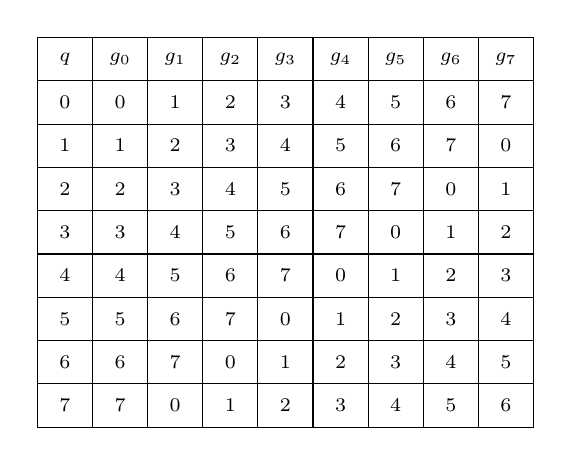
\begin{tikzpicture}[font=\scriptsize]
\matrix (m) [matrix of nodes,
  nodes={draw,minimum width=7mm,minimum height=5.5mm,anchor=center},
  row sep=-\pgflinewidth,column sep=-\pgflinewidth] {
  $q$ & $g_0$ & $g_1$ & $g_2$ & $g_3$ & $g_4$ & $g_5$ & $g_6$ & $g_7$ \\
  0 & 0 & 1 & 2 & 3 & 4 & 5 & 6 & 7 \\
  1 & 1 & 2 & 3 & 4 & 5 & 6 & 7 & 0 \\
  2 & 2 & 3 & 4 & 5 & 6 & 7 & 0 & 1 \\
  3 & 3 & 4 & 5 & 6 & 7 & 0 & 1 & 2 \\
  4 & 4 & 5 & 6 & 7 & 0 & 1 & 2 & 3 \\
  5 & 5 & 6 & 7 & 0 & 1 & 2 & 3 & 4 \\
  6 & 6 & 7 & 0 & 1 & 2 & 3 & 4 & 5 \\
  7 & 7 & 0 & 1 & 2 & 3 & 4 & 5 & 6 \\
};
\end{tikzpicture}
\caption{Illustrative normalized $K=8$ cyclic schedule for $b_0=0$ and positive orientation. Secret base and orientation permute the displayed labels while preserving the property that each coded symbol visits all eight clusters once per complete cycle.}
\Description{A nine-column matrix showing sessions zero through seven and a cyclic rotation of cluster labels zero through seven for eight Gray-ordered coded symbols.}
\label{fig:cyclic-map}
\end{figure}

For each required mapped label, the sender chooses one five-cover group using the signature-balanced keyed scheduler and transmits the five unchanged images. Each cover appears at most once inside one transmission. The receiver re-embeds each image, recovers five labels, takes their strict majority, inverts $\pi_q$, reconstructs the coded bitstream, applies Reed--Solomon decoding, and accepts plaintext after framing and AES-GCM verification.

\subsection{Finite-index feasibility}

For protected envelope $c$, let $d_k(c)$ denote the number of group occurrences required for label $k$ after coding and session mapping, and $a_k$ the number of available groups in label bank $k$. The session is feasible when
\begin{equation}
 d_k(c)\le a_k \quad \text{for every }k.
 \label{eq:feasible}
\end{equation}
Nominal alphabet capacity $\log_2 K$ gives coded bits per label, while Eq.~\eqref{eq:feasible} tests complete-message realizability under finite group availability and within-session unique-cover usage.

\subsection{Protocol properties and component roles}

Two exact properties hold before experimental evaluation. First, for any fixed coded symbol $v$ and any starting sequence $q_0$, the multiset $\{\pi_{q_0+t}(v):0\le t<K\}$ contains every cluster label exactly once because the additive shift traverses all residues modulo $K$ while Gray ordering and orientation permute fixed symbol positions. Second, under unique-cover usage and a preconstructed group bank, Eq.~\eqref{eq:feasible} is necessary and sufficient for emitting the complete coded session: each occurrence consumes one distinct group of its mapped label, and any feasible demand vector can be assigned distinct available groups label by label.

\begin{table}[t]
\caption{Role of the principal components and the evidence that supports each role.}
\label{tab:roles}
\small
\begin{tabularx}{\textwidth}{@{}lXX@{}}
\toprule
Component & Protocol role & Evidence/guarantee \\
\midrule
Calibration-locked projection & Define an externally fixed $K=8$ label space & Selection uses calibration attacks; holdouts remain reserved for validation \\
Complementary five-cover bank & Convert heterogeneous per-cover failures into majority decisions & Group failure signatures and 1,800/1,800 external calibration recoveries \\
RS128 & Correct residual coded-byte errors & Up to 37 corrections in calibration and 64 on holdout crop \\
Cyclic keyed Gray map & Balance coded-symbol-to-cluster assignment & Exact $K$-session algebraic balancing property \\
Signature-balanced scheduler & Preserve calibration-failure-signature mixture during keyed selection & Proportional-deficit scheduling followed by independent detector audit \\
AES-GCM + sequence/replay state & Authenticate accepted plaintext and session metadata & Standard AEAD semantics, explicit nonce discipline, stateful replay rejection \\
\bottomrule
\end{tabularx}
\end{table}

Table~\ref{tab:roles} isolates component roles and evidence types. The manuscript evaluates the integrated frozen protocol, while component-removal causal studies remain a natural extension for future work.

\section{Experimental Design}
\label{sec:experiment}

\subsection{Development/external split}

BOSSBase 1.01 (10,000 512$\times$512 grayscale images) is the development corpus used to choose the final protocol family and operating point. It is therefore not used as untouched external evidence in the headline TOMM claims. External validation uses the official Caltech-101 distribution, containing 9,144 readable source images. For each seed in $\{11,29,47,71,101\}$, a deterministic permutation assigns 1,500 images to descriptor training and the next 7,000 disjoint images to the cover index. Caltech images are converted uniformly to RGB before the 256$\times$256 channel fit.

The frozen external operating point is $K=8$, group size five, 128 parity bytes, and 30 authenticated sessions per partition. Ten deterministic plaintexts are generated at each of 8, 32, and 64 bytes; global authenticated sequences are 0--9, 10--19, and 20--29 respectively. A public deterministic benchmark root derives partition-specific keys and nonces, so the experiment is reproducible while making no production key-management claim.

\subsection{Calibration and holdout channel tests}

The twelve calibration transformations are exactly those listed in Section~\ref{sec:method}. The holdout set is never used for projection or group-bank construction and contains eight intermediate/stronger transformations: Gaussian noise 9 and 15; blur 1.2 and 1.8; central crop 8\% and 12\%; and rotations 5 and 9 degrees. Each of 30 sessions is evaluated under every transformation for each of five partitions, yielding 1,800 calibration trials and 1,200 holdout trials. Trial success requires exact authenticated plaintext recovery; a high symbol-accuracy value without successful AEAD verification is a failure.

\subsection{Selection-detectability audit}

The final detector audit reconstructs the complete 30-session selected-cover schedule for every external partition. For each partition and each of 20 repetitions, a 65/35 image-disjoint train/test split is created with split seed $10{,}000s+r$. The same split is used across all 30 session heads. We report macro-AUC across heads for three frozen detectors:

\begin{enumerate}
\item a 52-dimensional residual/SRM-lite representation with a native multi-output ExtraTrees classifier (300 trees, square-root feature sampling, balanced classes);
\item five GLCM texture features with standardized balanced logistic regression, trained independently for each session head;
\item a lightweight 30-output CNN trained for eight epochs with AdamW ($10^{-3}$, weight decay $10^{-4}$), batch size 32, and binary cross-entropy with logits.
\end{enumerate}

There are 100 repeated splits per detector. Because splits overlap within a partition, intervals over those repetitions are descriptive rather than confirmatory independent-sample confidence intervals; we do not report a naive one-sample repeated-split $t$-test.

\subsection{Frozen DiffStega reproduction}

DiffStega \cite{yang2024diffstega} is executed from official commit \texttt{73cd7cb8d102f4fc0f5bb168a71cfb948077d89a} on the official 100-case UniStega corpus (30 similar-prompt, 42 content-prompt, 28 style-prompt cases). The environment uses Python 3.11.5, PyTorch 2.1.0+cu121, CUDA 12.1, and a Tesla T4. All upstream benchmark commands and model identifiers remain frozen. The benchmark produces 700 PNG files and no evaluation error.

The upstream repository does not provide the metric-extraction scripts used for its paper tables. We therefore compute PSNR, SSIM, LPIPS, face ID similarity where applicable, CLIP score, and NIQE in an independent post-execution metric environment. Two package versions in that metric-only environment differ from the preregistered freeze (\texttt{huggingface-hub} 0.36.2 vs. 0.20.3 and \texttt{pyiqa} 0.1.15 vs. 0.1.13). Consequently, these are labeled \emph{independently reproduced metrics}; exact equality with the IJCAI table is neither expected nor claimed.

\section{Results}
\label{sec:results}

\subsection{External calibration feasibility and recovery}

All five external partitions produce feasible group banks for all 30 authenticated sessions. Across five partitions, 30 sessions, and 12 calibration attacks, all 1,800 protected messages are recovered and authenticated. Maximum Reed--Solomon corrections in any calibration trial are 37, below the 64-byte correction radius implied by 128 parity bytes. Every 7,000-cover index is exercised over the complete schedule, which avoids the trivial security failure mode of permanently restricting communication to a small fixed subset.

\begin{table}[t]
\caption{External Caltech-101 calibration results under the frozen protocol. Projection selection uses calibration evidence only.}
\label{tab:calibration}
\small
\begin{tabular}{@{}rlrrr@{}}
\toprule
Seed & Selected projection & Stable covers & Recovery & Max RS corr. \\
\midrule
11  & random\_04 & 4,184 & 360/360 & 5 \\
29  & random\_04 & 3,795 & 360/360 & 37 \\
47  & random\_15 & 4,756 & 360/360 & 0 \\
71  & random\_20 & 3,933 & 360/360 & 11 \\
101 & random\_28 & 4,167 & 360/360 & 0 \\
\midrule
All & -- & -- & 1800/1800 & 37 \\
\bottomrule
\end{tabular}
\end{table}

\subsection{Unseen holdout robustness}

The external holdout campaign recovers 1,163 of 1,200 authenticated messages (96.92\%). Failure is sharply localized: all 37 failures occur under the unseen 12\% central crop. The other seven transformations each recover 150/150 messages. This localization matters more than the aggregate alone; it identifies cropping beyond the calibration range as the dominant external-validity boundary.

\begin{table}[t]
\caption{External holdout results. Cover-label accuracy is averaged before group majority/FEC; message success requires final authenticated plaintext recovery.}
\label{tab:holdout}
\small
\begin{tabular}{@{}lrrr@{}}
\toprule
Holdout transformation & Auth. recovery & Mean label acc. & Max RS corr. \\
\midrule
Gaussian $\sigma=9$  & 150/150 & 0.964 & 0 \\
Gaussian $\sigma=15$ & 150/150 & 0.950 & 2 \\
Blur 1.2              & 150/150 & 0.958 & 0 \\
Blur 1.8              & 150/150 & 0.928 & 5 \\
Crop 8\%              & 150/150 & 0.707 & 34 \\
Crop 12\%             & 113/150 & 0.603 & 64 \\
Rotate $5^\circ$      & 150/150 & 0.923 & 0 \\
Rotate $9^\circ$      & 150/150 & 0.860 & 26 \\
\midrule
All holdouts           & 1163/1200 & -- & 64 \\
\bottomrule
\end{tabular}
\end{table}

Per-partition authenticated success is 240/240, 214/240, 240/240, 231/240, and 238/240 for seeds 11, 29, 47, 71, and 101. Thus the strongest crop exposes partition variability even though seven other holdouts are uniformly recovered.

\subsection{Selection detectability}

Table~\ref{tab:detectors} and Fig.~\ref{fig:detectors} summarize the final detector audit. SRM-lite remains essentially at chance. GLCM reveals a small, highly repeatable texture/selection shift. The trained CNN is the strongest evaluated warden, with mean macro-AUC 0.5266; every seed-level mean lies above 0.523. This is a modest but systematic signal. It falsifies any universal ``undetectable'' characterization and motivates the narrower statement that NARCIS has low detectability under the evaluated matched-index detector family.

\begin{table}[t]
\caption{Final repeated Caltech-101 selection-detector audit ($n=100$ overlapping image-disjoint splits per detector). Intervals are descriptive, not independent-sample inferential confidence intervals.}
\label{tab:detectors}
\small
\begin{tabular}{@{}lrrrr@{}}
\toprule
Detector & Mean AUC & SD & Min--Max & Descriptive 95\% interval \\
\midrule
SRM-lite + ExtraTrees & 0.5040 & 0.0023 & 0.4969--0.5088 & 0.5036--0.5045 \\
GLCM + logistic       & 0.5128 & 0.0017 & 0.5088--0.5162 & 0.5125--0.5132 \\
30-head CNN           & 0.5266 & 0.0034 & 0.5186--0.5340 & 0.5259--0.5273 \\
\bottomrule
\end{tabular}
\end{table}

\begin{figure}[t]
\centering
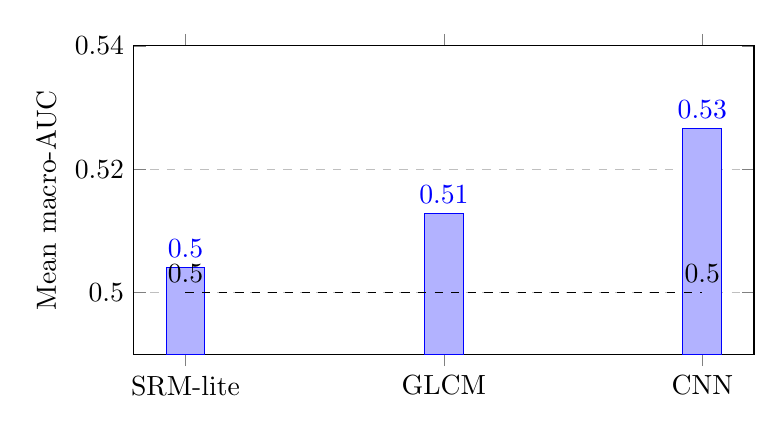
\begin{tikzpicture}
\begin{axis}[
  ybar,
  ymin=0.49,ymax=0.54,
  ylabel={Mean macro-AUC},
  symbolic x coords={SRM-lite,GLCM,CNN},
  xtick=data,
  bar width=14pt,
  width=0.78\textwidth,
  height=55mm,
  nodes near coords,
  nodes near coords align={vertical},
  ymajorgrids=true,
  grid style={dashed},
]
\addplot coordinates {(SRM-lite,0.504048) (GLCM,0.512833) (CNN,0.526603)};
\addplot[sharp plot,dashed,mark=none] coordinates {(SRM-lite,0.5) (CNN,0.5)};
\end{axis}
\end{tikzpicture}
\caption{Mean macro-AUC of the frozen detector battery. The dashed reference is chance AUC 0.5.}
\Description{Bar chart with SRM-lite at 0.504, GLCM at 0.513, and CNN at 0.527, with a dashed chance line at 0.5.}
\label{fig:detectors}
\end{figure}

\subsection{DiffStega reproduction and comparison boundary}

All 100 official UniStega cases complete under the frozen external execution. Table~\ref{tab:diffstega} compares the independently reproduced values with the published IJCAI reference. Correct-recovery PSNR is 23.274 dB, within 0.016 dB of the reported 23.290 dB. Face-ID similarity on 22 face cases is likewise close (0.888 vs. 0.893). Other metrics show larger offsets, which are retained rather than tuned away and are consistent with using an independent metric environment.

\begin{table}[t]
\caption{DiffStega external reproduction. ``Reproduced'' values are independently computed from the 100-case official execution; ``Published'' values are reported by Yang et al. \cite{yang2024diffstega}.}
\label{tab:diffstega}
\small
\begin{tabular}{@{}llrr@{}}
\toprule
Condition & Metric & Reproduced & Published \\
\midrule
Encrypted & PSNR & 18.569 & 18.611 \\
          & SSIM & 0.529 & 0.590 \\
          & LPIPS & 0.418 & 0.461 \\
          & Face ID similarity & 0.345 & 0.343 \\
          & CLIP score & 28.946 & 29.446 \\
          & NIQE & 3.901 & 3.408 \\
\midrule
Correct recovery & PSNR & 23.274 & 23.290 \\
                 & SSIM & 0.672 & 0.769 \\
                 & LPIPS & 0.183 & 0.266 \\
                 & Face ID similarity & 0.888 & 0.893 \\
\midrule
No password & PSNR & 18.495 & 18.491 \\
Wrong password & PSNR & 17.613 & 17.530 \\
\bottomrule
\end{tabular}
\end{table}

These values are not inserted into a ``NARCIS vs. DiffStega'' winner table. DiffStega's information object is a reconstructed secret image and its perceptual metrics quantify that reconstruction. NARCIS's primary outcome is exact authenticated recovery of a byte string from a finite natural-image index. Comparing PSNR with NARCIS's symbol rate or treating the two as equal-capacity systems would therefore be a category error.

\section{Discussion}
\label{sec:discussion}

\subsection{What the external evidence establishes}

The calibration result shows that a single frozen protocol transfers across five Caltech partitions without partition-specific changes to $K$, group size, parity, projection ranking, mapping, or detector settings. The holdout result goes further by exposing the channel boundary: moderate Gaussian noise, blur, 8\% crop, and 9-degree rotation remain fully recoverable at the authenticated-message level, whereas 12\% crop exceeds the error-correction margin in 37 trials. Reed--Solomon coding is therefore not a decorative component; crop 8\% requires as many as 34 corrected byte positions, and the strongest crop reaches the 64-position correction radius.

The group-bank mechanism also clarifies why individual-cover stability is not the only useful quantity. A five-cover group can remain majority-correct when member errors are complementary. This allows the final external schedule to use all 7,000 covers in every partition while still attaining perfect calibration recovery. The result supports the design principle that channel qualification can be performed at the decision unit actually transmitted---a group---rather than by retaining only covers that are individually invariant to every attack.

\subsection{Detectability as a separate security axis}

The detector hierarchy is informative. SRM-lite residual statistics do not find a practically meaningful separation, while GLCM detects a weak texture/selection shift and the CNN finds the strongest signal. This ordering is consistent with selection leakage being a distributional property rather than a pixel-embedding artefact. The result should not be softened into an undetectability claim. Under the tested matched-index warden, NARCIS is weakly but measurably detectable.

Conversely, AUC 0.527 is not evidence that an arbitrary Internet warden can recover payloads or even reliably flag single transmissions in a different deployment distribution. The experiment measures one explicit selected-vs.-remainder discrimination problem. It does not include sequence-level traffic features, temporal metadata, semantic profiling, or adaptive wardens trained after observing the secret selection key. Those are distinct threat models.

\subsection{Why the exact cyclic map matters}

Secret payload/framing bits are not guaranteed to be uniformly distributed at every finite message length. A fixed symbol-to-cluster permutation could therefore create persistent cluster-frequency skew even if group selection is balanced inside each cluster. The cyclic keyed Gray map removes that persistent assignment deterministically: over each full $K$-session cycle, each coded symbol visits every visual cluster exactly once. This property does not make the selected image distribution identical to the cover-index distribution, but it removes one avoidable source of repeated-session cluster bias before any empirical detector is run.

\subsection{Relation to recent coverless and generative work}

NARCIS and Guo--Ping address complementary priorities. Guo--Ping optimize robust/high-capacity mapping under their published datasets and attack protocol \cite{guo2026capacity}; NARCIS makes finite protected-message feasibility and authenticated recovery explicit, at a lower fixed alphabet $K=8$ in the external campaign. DiffStega demonstrates a different generative regime in which a secret image is reconstructed with diffusion models \cite{yang2024diffstega}. The faithful 100-case reproduction strengthens the empirical positioning because the comparator is executable, but the semantic mismatch prevents a responsible claim of numerical superiority.

\section{Limitations and Threats to Validity}
\label{sec:limitations}

\paragraph{External validity.} Caltech-101 is one external natural-image corpus. BOSSBase influenced method development and is therefore not counted as untouched confirmation. Validation on newer large native-resolution corpora, social-media recompression pipelines, and heterogeneous acquisition devices would test a broader domain.

\paragraph{Channel boundary.} Robustness is bounded to the declared transformations and strengths. The 12\% crop result is an observed failure boundary, not an outlier to discard. More severe cropping, perspective warps, arbitrary resampling chains, occlusion, color transformations, and learned image editing are not covered by the present claim.

\paragraph{Warden boundary.} The SRM-lite, GLCM, and CNN battery covers residual, texture, and learned selected-vs.-non-selected discrimination. It does not prove security against every steganalyzer or traffic-analysis adversary. Repeated-split intervals are descriptive because splits overlap.

\paragraph{Cryptographic boundary.} AES-GCM and HMAC are used as standard primitives; NARCIS does not introduce new cryptography. Benchmark key/nonce derivation is public reproducibility machinery, not a production KMS design. Cryptographic payload protection does not imply statistical secrecy of the carrier sequence.

\paragraph{Comparator boundary.} DiffStega is faithfully executed at its frozen upstream commit, but metric extraction is independent because the repository does not ship the paper's metric scripts. Two metric-only package versions differ from the preregistered versions. The resulting values are therefore reproduction diagnostics, not a claim of exact table replication.

\section{Reproducibility and Artifact Traceability}
\label{sec:repro}

The public NARCIS artifact records dataset provenance, frozen seeds, checkpoint hashes, calibration/holdout protocols, group-bank construction, exact session mapping, detector schedules, raw detector tables, workflow identifiers, DiffStega commit/model revisions, commands, output manifests, and SHA-256 hashes. Canonical manuscript-facing numerical results are generated from machine-readable files in \texttt{tomm\_results/}. The DiffStega evidence bundle has SHA-256 \texttt{32d0e975eb197adb0d1d2f7c537b04b4fab84af45a51148eaf15872b40de1f46}. The external detector CNN workflow completed 20/20 jobs and persisted 3,000 per-head AUC rows plus 100 repetition-level macro-AUC rows. BOSSBase development summaries, Caltech calibration/holdout aggregates, detector summaries, and DiffStega reproduction summaries are versioned alongside the protocol freezes.

The code repository is \url{https://github.com/EkodeckStephane/NARCIS}. The submission snapshot records the final title, author order, manuscript sources, bibliography, and canonical evidence lineage used for every headline number.

\section{Conclusion}
\label{sec:conclusion}

NARCIS formulates selection-based coverless image communication as a finite-index authenticated signaling problem. Its final protocol combines a learned invariant descriptor, calibration-locked $K=8$ quantile codebooks, complementary five-cover group banks, signature-balanced keyed selection, exact cyclic Gray cluster balancing, AES-GCM authenticated sessions, replay control, and Reed--Solomon correction.

The completed evidence stack spans development, external robustness, selection detectability, and executable baseline reproduction. Across five BOSSBase development seeds, the frozen K=8 lineage reaches 1,800/1,800 calibration recoveries while exercising 7,995--8,000 covers per seed. Across five externally frozen Caltech-101 partitions, all 1,800 calibration messages authenticate and every 7,000-cover index is exercised. The 1,200 unseen holdout trials yield 1,163 authenticated recoveries (96.92\%); seven transformations achieve 150/150 and the 12\% crop yields 113/150, defining the strongest observed channel boundary. Final mean macro-AUCs are 0.504 for SRM-lite, 0.513 for GLCM, and 0.527 for the trained CNN, supporting a low measurable selection-leakage characterization. The frozen 100-case DiffStega execution completes all cases and reproduces correct-recovery PSNR at 23.274 dB versus 23.290 dB in the reference paper.

These results establish a reproducible operating point with strong bounded channel robustness, explicit finite-index feasibility, complete-index participation, authenticated recovery, and detector-scoped security evidence. The next research frontier is stronger geometric resilience together with further reduction of learned selection leakage across broader external image domains and deployment wardens.


\bibliographystyle{ACM-Reference-Format}
\bibliography{narcis_core,tomm_positioning,external_comparators}

\end{document}
